\chapter{Workbook Assignment 1: Basic Probabilities and Visualisations}

\section{Bernoulli Distribution}
For each of the distributions below, please provide the requested graphics as well as the numeric results. In both cases, please provide how you realized these (calculations, code, steps…) and why it is the appropriate tools. Do not forget to include the scale of each graphics so a reader can read the numbers represented.

\section{Bernoulli Distribution}

Assumed a binary vote with outcome for or against is described by a Bernoulli distribution, with $P(vote = "for") = 0.69$. 
Interpreting this as a one-trial Bernoulli experiment with the two outcomes for and against - represented by success and no success respectively - we can visualize it as displayed in figure~\ref{fig:1a}.


\begin{figure}[h]
\centering
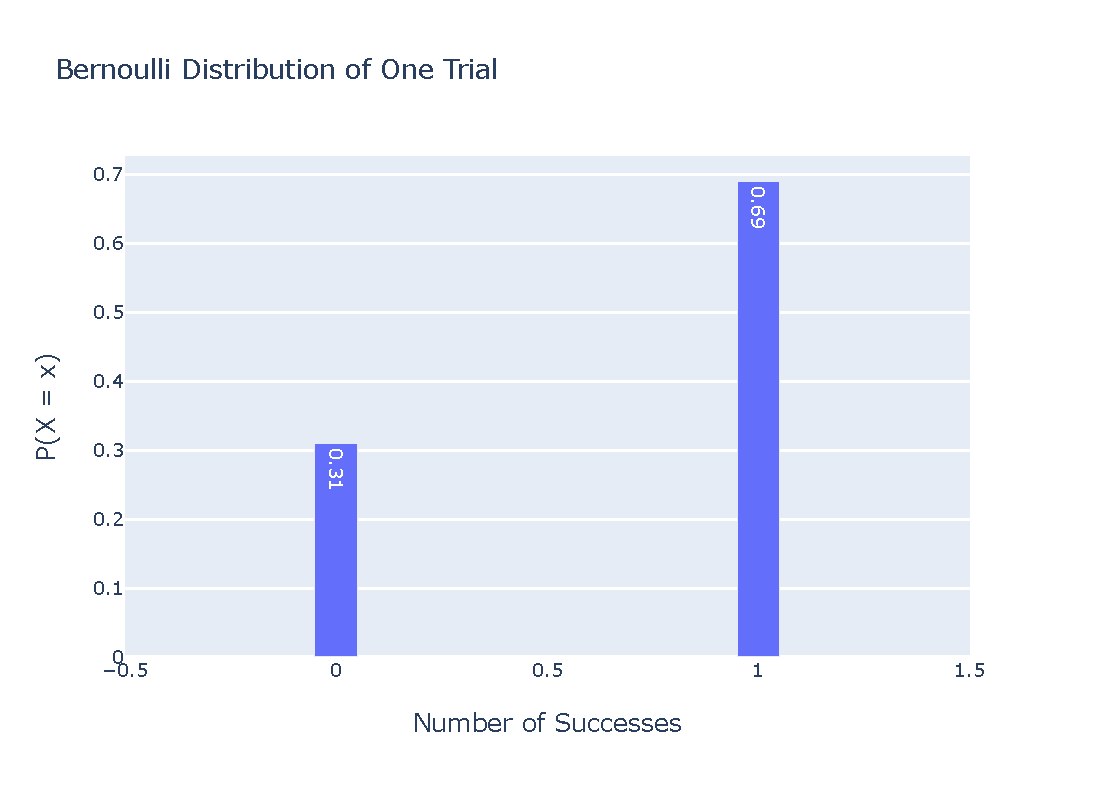
\includegraphics[width=16cm]{pics/1a.pdf}
\caption{Bernoulli distribution of one trial}
\label{fig:1a}
\end{figure}
\FloatBarrier


As this is a one-trial Bernoulli experiment, we can only observe the two outcomes $success = for$ and $no~success = against$. With provided information that $P(vote = "for") = 0.69$, we can calculate that $P(vote=”against”) = 1 - P(vote = "for") = 0.31$. This is visualized by the two bars in figure~\ref{fig:1a}. Following Hogg et al. \cite[Chapter~3.1]{hogg}, the expected value of X, described by a Bernoulli Distribution, is: 

\begin{equation}  \mu = E(X) = (0)(1-p) + (1)(p) = p
\label{eq:expvaluebernoulli}\end{equation}

Applied to our problem,  $ \mu = p = P(vote = "for") = 0.69 $.

This means if we would repeat the experiment one hundred times, we expect to observe 69 successes. 


This result was achieved using Python 3.9 and the following code:

\begin{lstlisting}
from scipy.stats import bernoulli
import numpy as np
import pandas as pd
import plotly.express as px
import plotly.graph_objects as go
from plotly.subplots import make_subplots

#Dataset creation. Done manually as only one trial
p_for = 0.69
p_against = 0.31 #p_against = 1-p_for
df = pd.DataFrame([[1,p_for],[0,p_against]])

#Visualisation
trace1 = go.Bar(x = df[0],y = df[1],width = 0.1,text = df[1], 
    textposition = 'auto')
fig = make_subplots(x_title = 'Number of Successes',y_title = 'P(X = x)')
fig.add_trace(trace1)
fig.show()
fig.write_image("figures/1a.pdf")
\end{lstlisting}

\section{Poisson Distribution}

Assumed we try to model the number of meteorites falling on an ocean each year - why would a Poisson Distribution be a natural candidate?


The Poisson distribution is a discrete probability distribution representing the number of events occurring in a defined period. It assumes the events occur with a known constant mean rate and that the events are independent of the time since the last event \cite[Chapter~4.6]{illowsky2018introductory}. By definition, a pure Poisson distribution assumes that the variance $\sigma^2$ is equal to the mean $\mu$: $\sigma^2 = \mu$. Citation By using a Gamma-Poisson distribution however can lift this restriction. 

The event of a meteor impacting the world in a given year fulfills all requirements for such distribution. The event itself is of discrete nature as you cannot have a fractional count of impacts, and we assume meteorite impacts occur with a known constant mean rate and the impacts themselves are independent of the time since the last event. We do not know, whether the variance of the distribution is equal to the mean, but even if it was, we could relax this assumption by using the Poisson-based Gamma-Poisson distribution. For this exercise, we assume $\sigma^2 = \mu$. 

Additionally assuming $\mu = 64$ allows for an exemplary visualisation as in figure \ref{fig:1b}.

\begin{figure}[h]
\centering
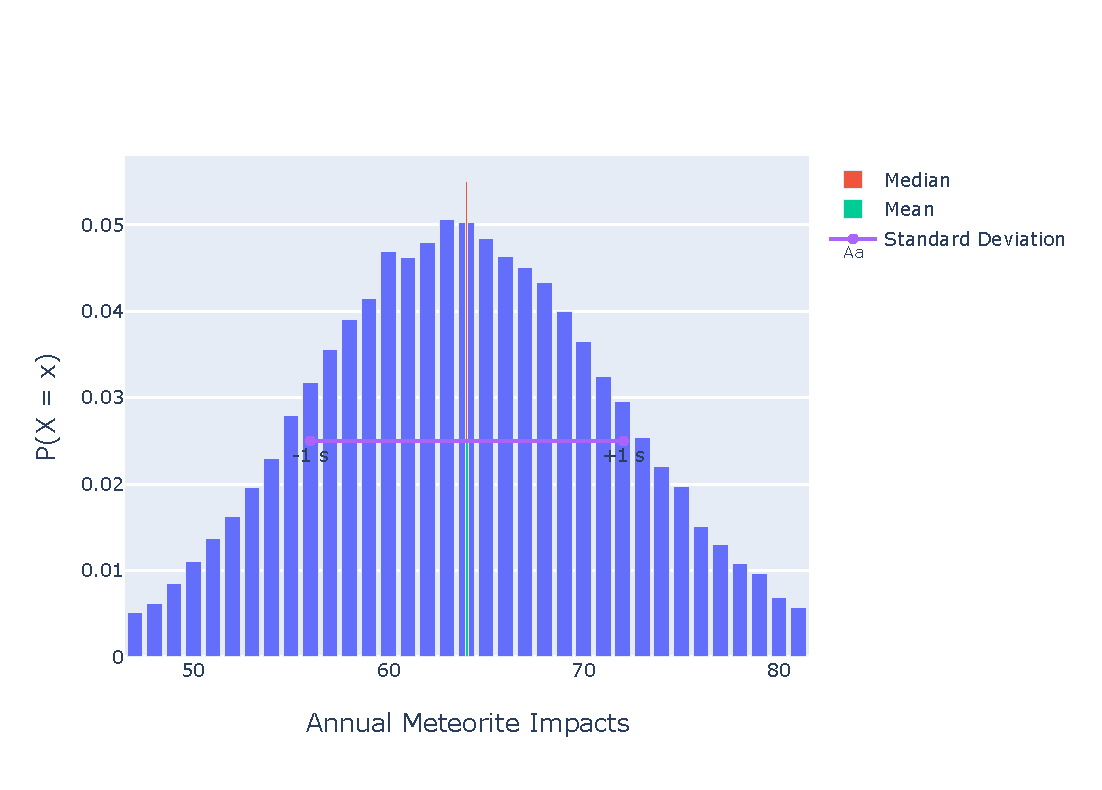
\includegraphics[width=16cm]{pics/1b.pdf}
\caption{Poisson distribution of annual meteorite impacts with $\mu = 64$}
\label{fig:1b}
\end{figure}
\FloatBarrier

To ensure readability of the graphic, probabilities $<0.5$ percent are excluded. Additionally, the variance ($s^2 = 64.36$) is visualised as its root, the sample standard deviation $s$ ($s = 8.02$). Looking at mean ($\bar{x} = 64.01$) and median ($m = 64$), one can barely see a difference, which is to be expected as the distribution displayed is not skewed. 

The calculations for this exercise were done in Python 3.9 with the following code: 

\begin{lstlisting}
from scipy.stats import poisson
import numpy as np
import pandas as pd
import plotly.graph_objects as go
from plotly.subplots import make_subplots

#creating a sample with fixed random state
size = 100000
raw = pd.Series(data = poisson.rvs(64, size=size, random_state = 42))

# calculating median, mean, variance, stdev
median = raw.median()
var = raw.var()  # sample assumed
mean = raw.mean()
stdev = np.sqrt(var)
stdev_range = pd.DataFrame([[raw.mean() - stdev, 0.025],
                            [raw.mean() + stdev, 0.025]])

# Filter to only display probabilities >=0.5%
df = pd.DataFrame(raw.value_counts())
df[0] = df[0].div(size)
df = df[df[0] >= 0.005]

# Display measures
print(var)
print(stdev)
print(mean)
print(median)

#creating graphic
trace1 = go.Bar(x = df.index, y = df[0],showlegend = False)
trace2 = go.Bar(x = [median], y = [0.055],width = [0.1], name = 'Median', 
text = [median], textposition = 'outside')
trace3 = go.Line(x = stdev_range[0], y = stdev_range[1], 
name = 'Standard Deviation', text = ['-1 s', '+1 s'],
mode ="lines+markers+text",textposition = "bottom center")
trace4 = go.Bar(x = [mean], y = [0.025],width = [0.15], name = 'Mean', 
text = [mean], textposition = 'outside')

fig = make_subplots(x_title = 'Annual Meteorite Impacts',
y_title = 'P(X = x)')
fig.add_trace(trace1)
fig.add_trace(trace2)
fig.add_trace(trace4)
fig.add_trace(trace3)
fig['layout'].update(barmode = 'overlay')
fig.show()

fig.write_image("figures/1b.pdf")
\end{lstlisting}

\section{Exponential Distributions}
Assuming the probability that you need to wait more than the random variable of y hours to hear a owl from your room is described by:

\begin{equation}  f(Y > y) = 0.2\overline{8}\mathrm{e}^{-0.5y} + 0.7\overline{1}\mathrm{e}^{-0.25y}
\label{eq:initcdf}
\end{equation}
To facilitate calculations, we reformulate the periodic numbers to fractions:

\begin{equation}  f(Y > y) = \dfrac{13}{45}\mathrm{e}^{-0.5y} + \dfrac{32}{45}\mathrm{e}^{-0.25y}
\label{eq:initcdffractioned}
\end{equation}

Suspecting that such events are usually exponentially distributed, we reformulate the probability in equation \ref{eq:truecdf} to the conventional expression \cite{deisenroth}. 

\begin{equation}  F_Y(y) = f(Y \leq y) =1-\left( \dfrac{13}{45}\mathrm{e}^{-0.5y} + \dfrac{32}{45}\mathrm{e}^{-0.25y} \right)
\label{eq:truecdf}
\end{equation}

As $Y$ and $y$ are defined as time and time cannot be negative, the domain of the function we are interested in is $[0,+\infty]$.

\begin{equation} f'_Y(y) = f''(Y \leq y) = 
\dfrac{-8\mathrm{e}^{-\frac{y}{4}}-13\mathrm{e}^{-\frac{y}{2}}}{180}
\label{eq:secderivative}
\end{equation}

As \ref{eq:secderivative}, the second derivative of formula \ref{eq:truecdf},  additionally has no real-valued solution for $y=0$, we can describe $F_Y(y)$ of \ref{eq:truecdf} as being upwards continuous monotonic increasing. Furthermore, $\lim_{y\to\infty} F_Y(y)= 1$ and $F_Y(y)= 0$ for the support of $y$. This is sufficient evidence to assume that the provided distribution of the random variable $y$ is a cumulative distribution function (CDF) of the family of exponential distributions. 

\begin{figure}[h]
\centering
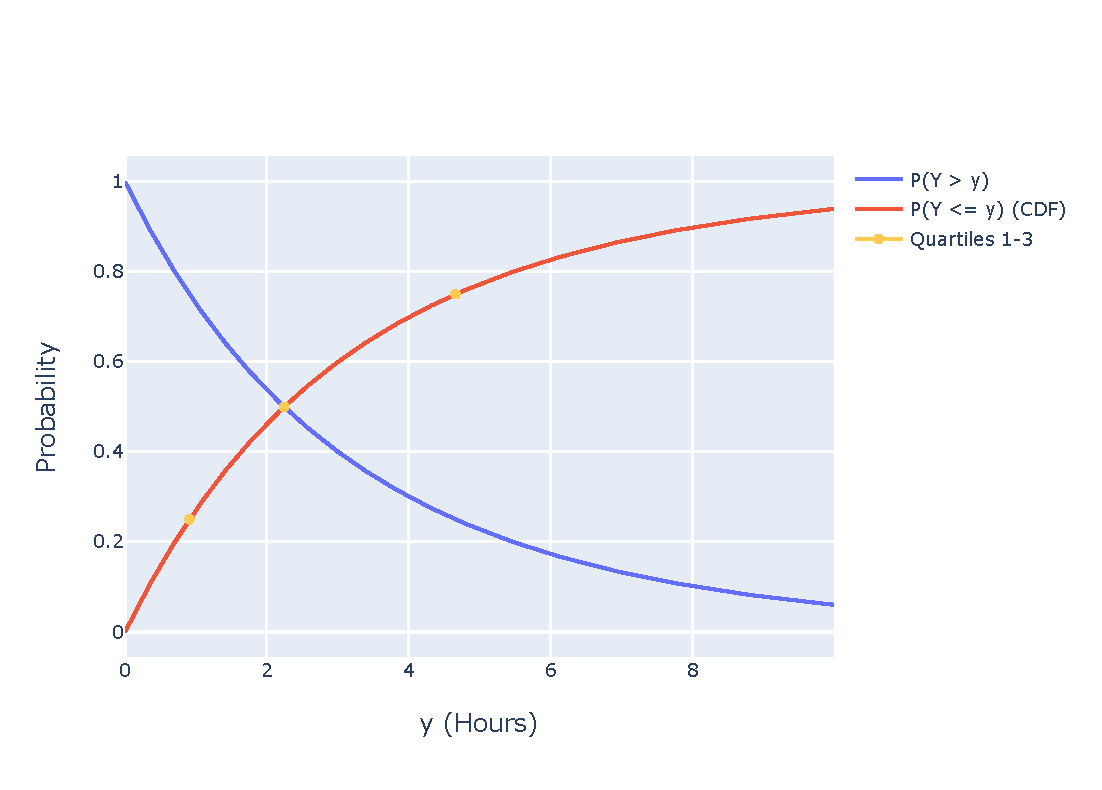
\includegraphics[width=16cm]{pics/1c1.pdf}
\caption{Visualisation of provided and reformulated CDF of task assignment}
\label{fig:1c1}
\end{figure}
\FloatBarrier


For any calculation regarding the probability to hear an owl within a time interval, we use the CDF. If we for example wanted to know $P(2 \leq Y \leq 4)$, the probability of needing to wait two to four hours to hear an owl, we would calculate it as described in equation \ref{eq:prob24}.

\begin{equation} P(2 \leq Y \leq 4) = P(Y \leq 4) - P(Y \leq 2)
\label{eq:prob24}
\end{equation}
%evtl explanation warum das so ist
Applied to our distribution, we calculate
\begin{equation} P (2 \leq Y \leq 4) =1-\left( \dfrac{13}{45}\mathrm{e}^{-2} + \dfrac{32}{45}\mathrm{e}^{-1}\right) -\left[ 1-\left( \dfrac{13}{45}\mathrm{e}^{-1} + \dfrac{32}{45}\mathrm{e}^{-0.5}\right)\right] 	\approx 0.23688696
\label{eq:probcalc24}
\end{equation}
Consequently, we can say that in 23.69 percent of cases, we have to wait in between two and four hours to hear an owl.
\\

Next to the CDF, we are also often interested in the corresponding probability density function (PDF). Generally, the PDF $f_Y(y)$ of a CDF $F_Y(y)$ is given by its first derivative \cite[Chapter~4.3]{montgomery2010applied}:
\begin{equation}
f_Y(y) = \frac{df(Y \leq y)}{dy}
\label{eq:firstderivative}
\end{equation}
For our CDF, the PDF is described by:
\begin{equation}
f_Y(y) = \dfrac{16\mathrm{e}^{-\frac{y}{4}}+13\mathrm{e}^{-\frac{y}{2}}}{90}
\label{eq:pdf}
\end{equation}

\begin{figure}[h]
\centering
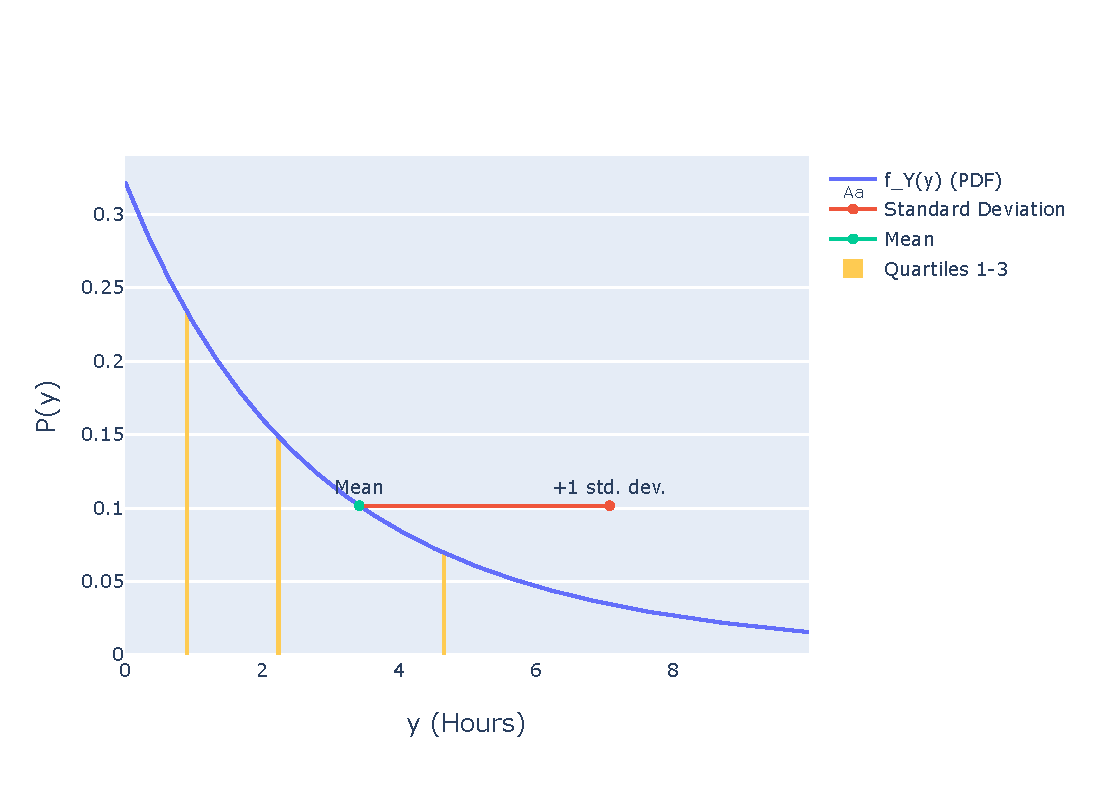
\includegraphics[width=18cm]{pics/1c2.pdf}
\caption{Visualisation of $f_Y(y)$ (PDF), the first two moments and applicable quartiles}
\label{fig:1c2}
\end{figure}
\FloatBarrier

The graphical representation of the PDF in figure \ref{fig:1c2} also includes the mean value. This is calculated using equation \ref{eq:ExpValueHogg} following the definition of an expectation for a random variable in Hogg et al. \cite[Definition~1.8.1]{hogg}.
\begin{equation}
E(X) = \int^{+\infty}_{-\infty} x f_X(x) ~ dx
\label{eq:ExpValueHogg}
\end{equation}
Conditions for this to be true are that equation \ref{eq:ExpValueHoggcondition} is fulfilled and that $X$ is a continuous random variable with $f_X(x)$ as its PDF.
\begin{equation}
\int^{+\infty}_{-\infty} |x| f_X(x) ~ dx < \infty
\label{eq:ExpValueHoggcondition}
\end{equation}
By the task assignment, we know that $y$ is a continuous random variable. By equation \ref{eq:pdf}, we calculated $f_Y(y)$ as the PDF of $y$. Lastly, as $y \in [0,\infty)$, equation \ref{eq:ExpValueHoggcondition} reduces to the right hand side of equation \ref{eq:ExpValueHogg} and the lower limit of the integral changes to 0. Consequently, if the mean or expected value $E(Y) < \infty$, it is valid. The calculation for our random variable $y$ in \ref{eq:ExpValueCalculation} returns $E(Y) < \infty$, we can therefore accept $3.4\overline{2}$ hours as our expected value $E(Y)$ for the waiting time to hear an owl. 
%
\begin{equation}
E(Y) = \int^{+\infty}_{0} y f_Y(y) ~ dy = \int^{+\infty}_{0} y\left(\dfrac{16\mathrm{e}^{-\frac{y}{4}}+13\mathrm{e}^{-\frac{y}{2}}}{90} \right) ~dy = \frac{154}{45} = 3.4\overline{2}
\label{eq:ExpValueCalculation}
\end{equation}
Following Hogg et al., the first moment or mean $\mu = E(X)$, if $X$ is a random variable with existing expectation \cite[Definition~1.9.1]{hogg}. This is the case for $Y$. Consequently, we can also assume that the mean value $\mu = 3.4\overline{2}$. 
\\

To calculate the second moment, the variance $\sigma^2$, we use definition 1.9.2 by Hogg et al. \cite{hogg} as equation \ref{eq:HoggVariance}.
\begin{equation}
\sigma^2 = E(X^2) - \mu^2
\label{eq:HoggVariance}
\end{equation}
%
The variance of $y$ is calculated by \ref{eq:YVariance}, using the same assumptions as for equation \ref{eq:ExpValueCalculation}.
\begin{equation}
\sigma^2 = \int^{+\infty}_{0} y^2 f(y) ~ dy - \mu^2
= \int^{+\infty}_{0} \dfrac{y^2\left(16\mathrm{e}^{-\frac{y}{4}}+13\mathrm{e}^{-\frac{y}{2}}\right)}{90} - \left(\frac{154}{45}\right)^2
= \frac{27044}{2025} \approx 13.3551
\label{eq:YVariance}
\end{equation}

The variance is also depicted in figure \ref{fig:1c2}     as its root, the standard deviation $\sigma \approx 3.6545$. 

Both figures \ref{fig:1c1} and \ref{fig:1c2} furthermore display the first three quartiles of the PDF. 


\chapter{Workbook Assignment 2: Basic Probabilities and Visualizations }	

\section{Visualisation, Expectations and (Co)Variances}
Assumed you have recorded mappings of X and Y values, what is an appropriate way of visualisation and how do you find the sample covariance as well as the expectation values and variances per variable; assuming the data comes in the following format?\\
\\
(1.754, 720.15), (-7.385, -260.86), (1.396, -340.56), (-3.304, 954.75), 
(-12.159, -370.12),\\ (-6.767, -259.89), (1.233, 261.89), (-7.056, 400.72), 
(-1.222, -94.33), (-0.722, -492.02),\\ (-5.065, -789.42), (-9.333, 301.86), 
(7.27, -17.04), (-1.989, 257.91), (3.582, -229.89), \\(-1.2, -349.18), 
(4.118, 226.05), (-1.834, -534.54), (-1.882, 610.91), (8.677, 70.11) \\

As the variables in the data are both continuous and the question addresses the calculation of correlation, the optimal visualisation is a scatter diagram as for example figure~\ref{fig:WorkbookAssignment2a}.

\begin{figure}[h]
\centering
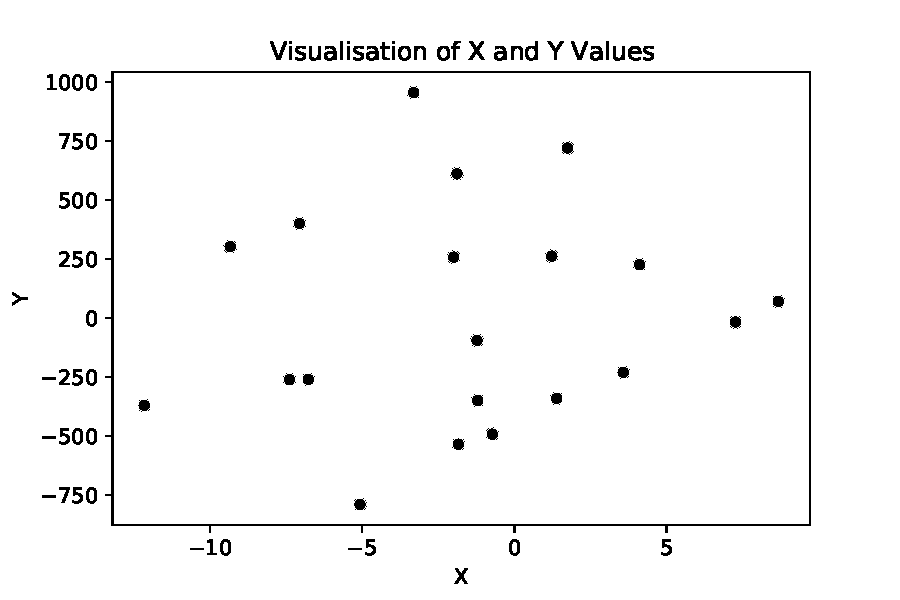
\includegraphics[width=16cm]{pics/WorkbookAssignment2a.pdf}
\caption{Visualisation of provided X and Y values as scatter plot}
\label{fig:WorkbookAssignment2a}
\end{figure}
\FloatBarrier

Looking at the scatter plot, one can observe that the data is quite evenly dispersed; No pattern can be determined at first glance. This rather evenly distributed data also suggests that the expected value for X and Y is rather close to 0. Calculating the expected value for each variable can be understood at the calculation of the expected value of a discrete random variable as the number of observations is discrete. Equation~\ref{eq:ExpValDiscrete} is therefore the formula to calculate the expected value. 


\begin{equation}  E(X) = \sum [x * P(x)]
\label{eq:ExpValDiscrete}
\end{equation}

http://mathcenter.oxford.emory.edu/site/math117/expectedValueOfADiscreteRandomVariable/
\\

The results are consequently $E(X) = -1.5944$ and $E(Y) = 3.3250$.

The sample covariance is defined in Equation~\ref{eq:COV}, where $\bar{x} = E(X)$ and $\bar{y} = E(Y)$ (adapted from~\cite{bruce2017practical}).

\begin{equation}  s_{xy} = \frac{\sum(x_{i}-\bar{x})(y_{i}-\bar{y})}{n-1}
\label{eq:COV}
\end{equation}

Applying the formula to the provided data, $s_{xy} = 284.23$ can be observed. This indicates a positive relationship, but does not provide any information on its quality. 

The calculations were done using Python 3.9 and the following code:

\begin{lstlisting}
import numpy as np
import pandas as pd
import seaborn as sns
import matplotlib.pyplot as plt
data = (1.754, 720.15), (-7.385, -260.86), (1.396, -340.56), (-3.304, 954.75),
(-12.159, -370.12), (-6.767, -259.89), (1.233, 261.89), (-7.056, 400.72), 
(-1.222, -94.33), (-0.722, -492.02), (-5.065, -789.42), (-9.333, 301.86),
(7.27, -17.04), (-1.989, 257.91), (3.582, -229.89), (-1.2, -349.18), 
(4.118, 226.05), (-1.834, -534.54), (-1.882, 610.91), (8.677, 70.11)
data = pd.DataFrame(data)
data.columns = ["X", "Y"]
print("The variance of the variables is: \n{}".format(data.var()))
print("The expectation value for the variables is: \n{}".format(data.mean()))
print("The sample covariance is {}".format(data.cov().iloc[0,1]))

data = data.set_index("X")

sns.scatterplot(data = data, x = "X", y = "Y", color = "black").set(title = "Visualisation of X and Y Values")
plt.savefig('./figures/2a.pdf')
\end{lstlisting}


\section{Ball throw}
b) Consider that a ball is thrown with a random angle $THETA$[0,360) (in degrees) and a random radius $r$ element of [0,1] (in meters) both independent and uniform. Calculate the density of the variable $X$ and $Y$ (the cartesian coordinates of the point at angle $THETA$ and radius $r$) as well as their expectation and variance.

Notes:
Only possible by transformation. if you know x yy dirstribution 
Monte carlo approach can solve this. (complicated)
Transformation theorem thingy 3.last chapter
For density, check Page 19 in skript. basically the pdf of a distribution




\chapter{Workbook Assignment 3: A Simple Parameter Estimation}	
\chapter{Workbook Assignment 4: Hypothesis Test}	

Assumed we are producing high-quality hammers in our factory and want to model the production quality. From the last 1000 produced hammers, we observed an average weight of $\bar{x}=971~g$ and a standard deviation of $s=42~g$.

For modelling our distribution, the best proposal is a normal distribution. Hogg et al. \cite[Definition~3.4.1]{hogg} define the normal distribution as follows: 

\begin{equation} \frac{1}{{\sigma \sqrt {2\pi } }}e^{{{ - \left( {x - \mu } \right)^2 } \mathord{\left/ {\vphantom {{ - \left( {x - \mu } \right)^2 } {2\sigma ^2 }}} \right. \kern-\nulldelimiterspace}{2\sigma ^2 }}}
\label{eq:normaldist}
\end{equation}


It depends on two parameters, the population standard deviation $\sigma$ and the population mean $\mu$, which both are provided. In general, any normal distribution has a bell-shaped form, indicating that it is symmetric and not skewed to any side. Apart from the mean and the standard deviation, we are not provided any further data. Production inaccuracies are usually normally dispersed, and as we neither have access to the raw data of individual observations nor have information on any skewness or non-normal behaviour, a normal distribution is assumed - $ X~\sim~N(\mu, \sigma^2)$. This assumption of course does not hold anymore if the data of the 1000 produced hammers introduces any kind of bias or skewness. 


Other distributions are excluded as they are not applicable to this case or are less fitting. A Binomial Distribution for example is not applicable as it is binary, whereas the independent variable central to this exercise - hammer weight - is continuous. \\Describing the hammer weight as a repeated Bernoulli trial would also be an option to model the distribution, however such endeavor would firstly approximate a normal distribution as well and would secondly assume that the weight measurements are integer variables, whereas they are of continuous nature. \\
Another popular distribution, the Poisson distribution, is also not applicable as it models the average number of events per time interval \cite{bruce2017practical}. \\
Using an exponential distribution to model the weight dispersion of hammer production would imply that we expect for example continuously increasing counts of hammers for increasing weights, which is not a senseful assumption. \\
Consequently, we assume that the normal distribution is the best approximation.

Using the normal distribution as approximation implies accepting several assumptions. We assume that the model has the x-axis as an horizontal asymptote, that its mean is equal to its median, that its mode is the same as its mean and that it is symmetric about the mean \cite[Chapter~3.4]{hogg}.

Using \ref{eq:normaldist} with the provided parameters of $\mu = 971$ and $\sigma = 42$, the following model is proposed: 

\begin{equation} \frac{1}{{42 \sqrt {2\pi } }}e^{{{ - \left( {x - 971 } \right)^2 } \mathord{\left/ {\vphantom {{ - \left( {x - 971 } \right)^2 } {2(42) ^2 }}} \right. \kern-\nulldelimiterspace}{2(42) ^2 }}} ~~~=~~~ \frac{1}{{42 \sqrt {2\pi } }}e^{{{ - \left( {x - 971 } \right)^2 } \mathord{\left/ {\vphantom {{ - \left( {x - 971 } \right)^2 } {7056 }}} \right. \kern-\nulldelimiterspace}{7056 }}}
\label{eq:normaldistadapted}
\end{equation}

In \ref{eq:normaldistadapted}, we furthermore assume that we can use the provided values for the sample average and the sample standard deviation as population parameters $\sigma$ and $\mu$ as the sample size $n = 1000$ is large. 

Assumed we now test a new production system for hammer production. A random sample output of hammers of this new production output returns the following weights in grams: \\

\begin{center}
    1009, 1069, 966, 952, 1084, 897, 909, 995, 975, 983
\end{center}

How do we know if this new system's weight accuracy is better than the old system's accuracy, i.e. how do we find out whether the weight variance of the new system is lower than the variance of the old system?

To answer this question, we have to perform a statistical test comparing the variances of both samples. For this, we need to define our hypotheses. Overall, we want to reject the idea that the new system does not provide any reduction in weight variance. The hypotheses are consequently 
\\
\begin{center}
$H_0~~=~~ \sigma^2_2~<~\sigma^2_1$\\
$H_1~~=~~ \sigma^2_2~\geq~\sigma^2_1$
\end{center}
\\
where $\sigma^2_1$ is defined as the population variance of the old production system and $\sigma^2_2$ is defined as the population variance of the new production system.




-formulate Hypotheses\\
-what test\\
-what decision rule\\
-what p value/critical values\\
-do calculations




we can use the Central Limit Theorem as proven by Hogg et al. \cite[Theorem~5.3.1]{hogg}. 
If we now want to model the weight distribution of our hammers, the best assumption is a normal distribution. The 1000 produced hammers can be interpreted as a random sample of the population of hammers with $n = 1000$. This $n$ is $>30$, so the central limit theorem can be applied here. 



\chapter{Workbook Assignment 5: Sufficient Statistics}	
\chapter{Workbook Assignment 6: Bayesian Estimates}	

(following Hogg, McKean and Craig, exercise 11.2.2)
Let $X1, X2, ... , X10$ be a random sample from a gamma distribution with $\alpha =3$ and $\beta =1/\theta$. Suppose we believe that $\theta$ follows a gamma-distribution with $\alpha =3$ and $\beta = 2$

a) Find the posterior distribution of ��.
b) If the observed ��̅=16.5, what is the Bayes point estimate associated with the square-error loss function?
c) What is the Bayes point estimate using the mode of the posterior distribution?





\chapter{Latex}

\section{Tools}

MiKTeX: \url{https://miktex.org/download}
TeXLive: \url{http://tug.org/texlive/}
 (or alternative LaTeX-systems).
 
 A good editor is essential. Sometimes combined editors and compilers (e.g. TeXShop) can be really productive. Make sure you learn the use of synchronized navigation then.

A vector graphic is one where strokes remain strokes even at the highest resolutions: e.g. the Figure~\ref{fig:spiral} or the Logo on the \hyperref[titlePage]{Titelblatt} (notice: you can click from here to there).
Many tools generate vector-graphics for plots from any data-set. E.g. Plotly (with the use of the Browser-Print), MatPlotLib or even OpenOffice, LibreOffice or MS-Excel.

\section{Literature References}
Here is an example of a reference with a page-number: \cite[S. 6]{DueckKo:2016}


\section{Pictures}

\begin{figure}[h]
\centering
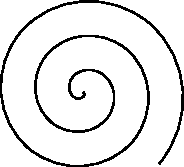
\includegraphics[width=8cm]{pics/spiral.pdf}
\caption{A spiral... smooth vector-based with a clean parametrisation! \\ Nothing to do with \cite{Gage:18}}\label{fig:spiral}
\end{figure}
\FloatBarrier

\section{Tables}

\begin{table}[H]
\small
\centering
\begin{tabular}{p{5cm}|l|p{3cm}}
`` Industrial era '' &  ``Jobs '' & `` Wanted: Upgrade''' \\ \hline
Parts exchanger & Fitter & mecatronics specialist \\
eShop & reseller & `` Client-suggester'' \\
`` Coding-guru''' & Softwaredesign & Whole-life designer \\
JA! Gut \& Günstig & brand-names & `` Life-Style Feeling'' \\
Internetbanking & Bank clerk & Customer adviser \\
Robots & Specialist & Machine supervisor \\
Bush & Gardener & Nature-sculptor \\
Painting & Painter & Interior Design \\
 &  & \\
\end{tabular}
\caption[Downgrade and upgrade of job denominations]{Downgrade and Upgrade of job denominations \\ \ \ \ \cite{DueckKo:2016}}
\label{tab:Downgrade and Upgrade of job denominations}
\end{table} 

\section{Listes}

\begin{itemize}
 \itemsep0pt
 \item one
 \item twoi
 \item threei
\end{itemize}

\begin{enumerate}
 \itemsep0pt
 \item first
 \item second
 \item third
\end{enumerate}


\section{Formulæ}

A formula can be written inline, e.g. as $ \frac{d}{dx}\mbox{arctg}(x) = \frac{1}{1+x^2}$ or, in centered math:

\begin{equation}  \frac{d}{dx}\mbox{arctg}(x) = \frac{1}{1+x^2} \label{arctanderivative}\end{equation}

Notice that formulæ that are centered start bigger (technically, they start in \verb+\displaystyle+) than they start inline (technically, they start in \verb+\textstyle+ all subsequents reductions, e.g. an exponent, goes to \verb+\scriptstyle+ then \verb+\scriptscriptstyle+). Indeed a best effort is made so that inline formulæ do not change the line height which would bother the eye of a reader.

Formulæ can be given a number and a label. Numbering happens automatically with \verb+\begin{equation}+ and \verb+\end{equation}+ and can be avoided if enclosing the formula betwee \verb+\[+ and \verb+\]+. If using the \verb+\label+ macro inside, you can refer automatically to this equation using \verb+\ref{label}+. E.g. Thanks to equation~\ref{arctanderivative} one dare say that:

\begin{equation} \int_0^t \frac{1}{1+x^2} dx = \mbox{arctan}(t) \end{equation}